\documentclass[aspectratio=169]{beamer}
\mode<presentation>
%\usetheme{Warsaw}
%\usetheme{Goettingen}
\usetheme{Hannover}
%\useoutertheme{default}

%\useoutertheme{infolines}
\useoutertheme{sidebar}
\usecolortheme{dolphin}


\setbeamersize{sidebar width left=0pt} % to remove the sidebar
\beamertemplatenavigationsymbolsempty % To remove the navigation symbols on the bottom right.
\setbeamersize{text margin left=10mm,text margin right=10mm} % Specify margins

\usepackage{amsmath}
\usepackage{amssymb}
\usepackage{listings}
\usepackage{enumerate}
\usepackage{hyperref}
\hypersetup{
    colorlinks=true,
    linkcolor=blue,
    filecolor=magenta,      
    urlcolor=cyan,
}
 
\urlstyle{same}

%some bold math symbosl
\newcommand{\Cov}{\mathrm{Cov}}
\newcommand{\Var}{\mathrm{Var}}
\newcommand{\brho}{\boldsymbol{\rho}}
\newcommand{\bSigma}{\boldsymbol{\Sigma}}
\newcommand{\btheta}{\boldsymbol{\theta}}
\newcommand{\bbeta}{\boldsymbol{\beta}}
\newcommand{\bmu}{\boldsymbol{\mu}}
\newcommand{\bW}{\mathbf{W}}
\newcommand{\one}{\mathbf{1}}
\newcommand{\bH}{\mathbf{H}}
\newcommand{\by}{\mathbf{y}}
\newcommand{\bolde}{\mathbf{e}}
\newcommand{\bx}{\mathbf{x}}

\newcommand{\cpp}[1]{\texttt{#1}}

%--------------------------------------------------
\providecommand{\abs}[1]{\lvert#1\rvert}
\providecommand{\norm}[1]{\lVert#1\rVert}
\providecommand{\Blue}[1]{\textcolor{blue}{#1}}
\providecommand{\Red}[1]{\textcolor{red}{#1}}
\newcommand{\celsius}{\ensuremath{^\circ}C}
\newcommand\thfore{\mathord{\therefore}\,}
%------------------------------------------------------------------

\title{Lecture 10. Binary Search Trees}
%\author{\includegraphics[width=.5\textwidth,height=.5\textheight]{lecture4-fig0.png}}

\date{ }
%------------------------------------------------------------------


\begin{document}

\frame[plain]{\titlepage}


\begin{frame}[plain]{Binary Search Tree}
 
  {\bf Example 10.1.} The custom dictionary in a spell-checker keeps track of words that 
     you don't want flagged as misspellings but aren't in the standard dictionary.
     These words get added one at a time, in no particular order, but it is necessary to keep them
     organized so that searching the list is easy.
     Suppose your custom dictionary contains the following words:
     
     \begin{center}
        {\small \bf macchiato, poset,  phat,  complexify,  jazzed,  sheafify, clueless}
     \end{center}

       What is an efficient way to organize this data? \pause 
       \medskip
       
    One possible organizational structure is a graph model called a \Blue{binary search tree}.
      \begin{itemize}
        \item Start with an item (chosen arbitrarily) at the top of the tree (root node).
        \item The root has (at most) two edges touching it, one going down to the right, and one going down to the left.
        \item The only condition is that the right child must come after its parent in alphabetical (or numerical) order,
        and the left child  must come before its parent.
      \end{itemize}

\end{frame}

\begin{frame}[plain]{ }
  \begin{itemize}[<+->]
   \item    The binary tree for the question is
   \medskip
   
    \begin{center}
         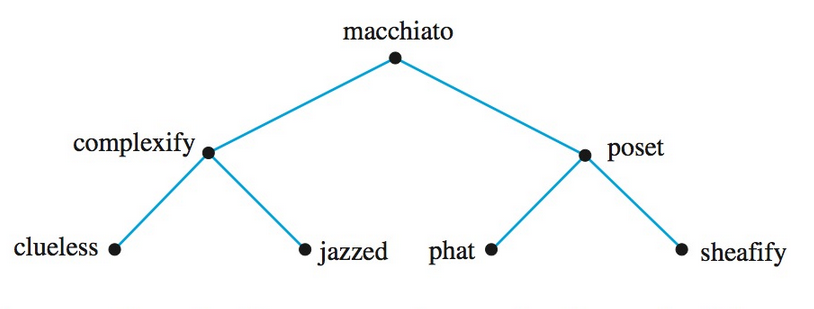
\includegraphics[height=3.7cm]{./img/lecture10-fig1.png}
       \end{center}
   \item For large data sets, the searching process in a binary tree structure
    goes very quickly since you don't need to look at
      every element. For example, to find ``poset'' in the tree, we only have to look at two words. To
       establish that ``iPod'' is not in the tree, we only need to check three words.
 \end{itemize}
\end{frame}


\begin{frame}[plain]{}

    {\small Each comparison moves the search one level down the tree, and
    each level containes twice the number of elements as the level before.
    For example, a balanced binary search tree within
    \[ 255 = 1+2+4+8+16+32+64+128 \]
    elements requires, at most eight comparisons to search it completely. }

    \begin{center}
        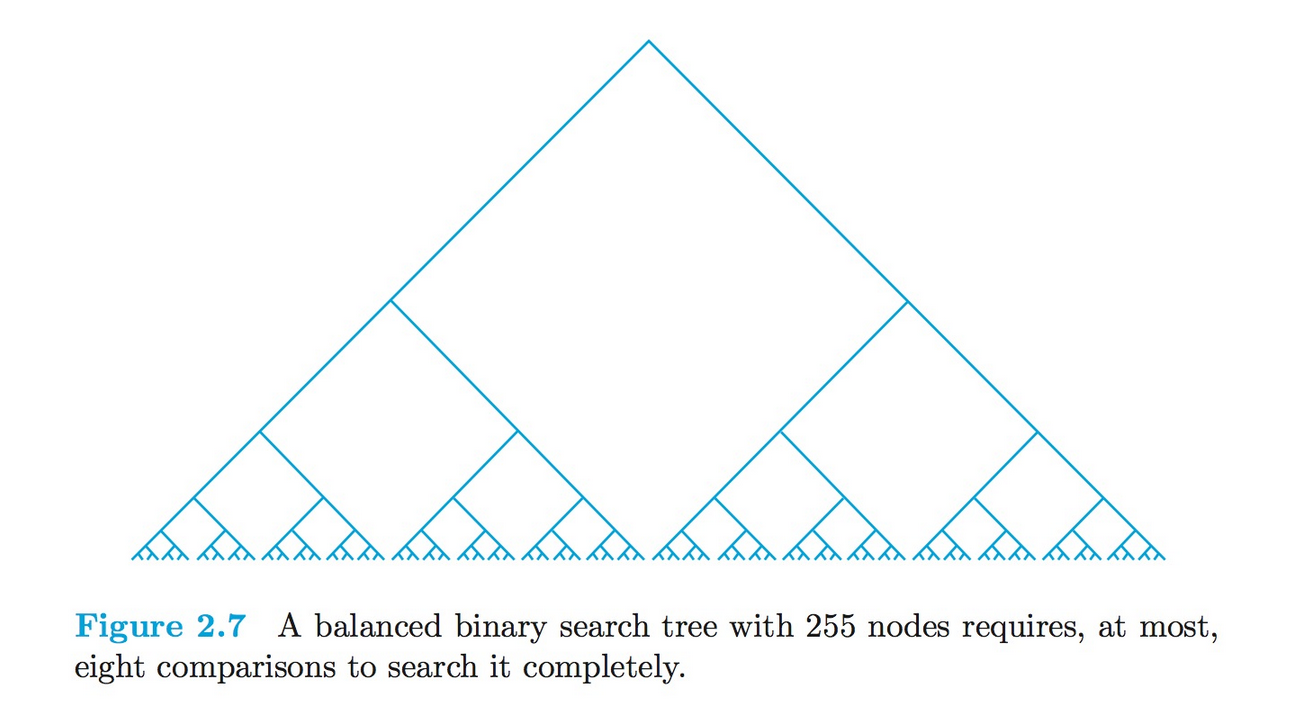
\includegraphics[height=5cm]{./img/lecture10-fig2.png}
      \end{center} 
  
\end{frame}


\begin{frame}[plain]{}

 {\bf Practice 10.2.}  Consider the following list of numbers.
     \[  123, 684, 121, 511, 602, 50, 43, 10, 320 \]
          
     \begin{itemize}
      \item[(a)] Place the list of numbers, \Red{in the order given},  
         into a binary search tree. (The organizing 
         condition is that the right child must come after its parent in
          numerical  order, and the left child must come before its parent.)
      \item[(b)] %The height of a binary search tree is the maximum number of edges you have to go 
        %through  to reach the bottom of the tree, starting at the root. 
        What is the height of the tree in part (a)? 
     \item[(c)] \Red{Reorder the numbers}\footnote{That is, choose a different number as a root.}
      so that when they are put into a binary search tree, 
        the height of the resulting tree is less 
     than the height of the tree in part (a). Give both your new list and the search tree it 
           produces.
    \end{itemize}
    
    \vspace{0.7in}
    
 \end{frame}
 
 
 \begin{frame}[plain]{Full and Complete Binary Trees}
 
 {\bf Definition 10.3.}  A \Blue{full binary tree}  is a  tree  in which every internal vertex
 has exactly two children. 
 \begin{center}
 \begin{tabular}{cc}
   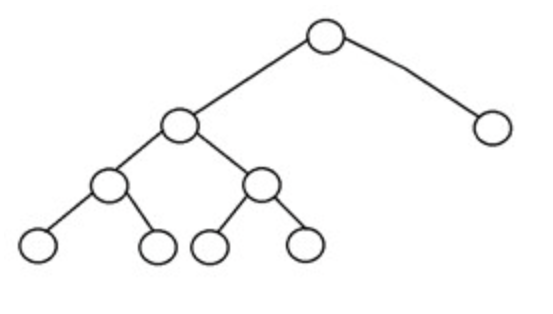
\includegraphics[height=2.3cm]{./img/lecture10-fig3.png}
   \end{tabular}
 \end{center}

 
 {\bf Definition 10.4.} A \Blue{complete binary tree}  is a binary tree in which every level, except possibly 
  the last,  is completely filled,  and the last level has all its vertices to the left side.
  
 \begin{center}
 \begin{tabular}{cc}
   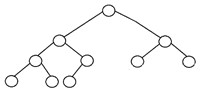
\includegraphics[height=2.2cm]{./img/lecture10-fig4.jpg}
   \end{tabular}
 \end{center}
  
 \end{frame}
 
 \begin{frame}[plain]{}
 
 \begin{center}
   \includegraphics[height=8cm]{./img/lecture10-fig5.png}
 \end{center}

 \end{frame}
 
 \begin{frame}[plain]{Perfect Binary Trees%~\footnote{Some authors use the term \Blue{complete}
 % to refer instead to a perfect binary tree 
 %and the term `complete' in Definition 10.5 is referred as an {\bf almost complete} or 
 %{\bf nearly complete} binary tree. } 
 }
 
 
 {\bf Definition 10.5.} A \Blue{perfect binary tree}  is a binary tree in which 
 all the internal vertices have strictly two children and every leaf  
 is at the same level or same depth within a tree. (i.e., a perfect tree = a complete full tree)
   
 \begin{center}
 \begin{tabular}{cc}
   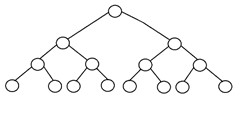
\includegraphics[height=2cm]{./img/lecture10-fig3.jpg}
   \end{tabular}
 \end{center}
 
 {\bf Theorem 10.6.} The number of vertices, $n(T)$,
  of a perfect binary tree having depth (or height) $h$ is $2^{h+1}-1$ :
 \[ \Blue{n(T) = 2^{h+1}-1} \]
 (Hint: $1, 2, 4, ..., 2^h$ is a geometric sequence. The sum of finite geometric series is
 $S_n = \frac{a_0(r^n-1)}{r-1}$ with $|r|>1$, where $n$ is the number of terms, $a_0$
 is the first term and $r\neq 1$ is the common ratio.)
  
 \end{frame}

 
 \begin{frame}[plain]{}
 
 How many items can a binary tree hold? \pause 
  Since a perfect binary tree of depth $h$ has $2^{h+1}-1$ nodes,
  
 \smallskip
 
 {\bf Theorem 10.7}
    The number of items that a binary tree (complete or not) can store is at most $2^{h+1}-1$. That is,
  \[ \Blue{n(T) \leq 2^{h(T)+1}-1} \]
 where $n(T)$ = the number of vertices on a binary tree $T$ and $h(T)$ = the height of $T$.
 \pause
\medskip

{\bf Exercise 10.8}. A binary tree $T_1$ has 100 vertices. 
Find the minimum and maximum possible heights of this tree.
\medskip


{\bf Exercise 10.9}. A second binary tree $T_2$ has height $h(T_2)=7$
and contains exactly $90$ vertices. Determine whether $T_2$ can be a complete
binary tree. Justify your answer.

\end{frame}

\end{document}
%%%%%%%%%%%%%%%%%%%%%%%%%

\begin{frame}[plain]{}

 {\bf Activity 10.8.}  Use {\bf Algorithm 1} to write a python code for
    inserting the word ``\emph{oceanography}" into the binary search tree in \emph{Example 10.1}.

    \begin{center}
      \includegraphics[height=6cm]{lecture10-fig5.png}
    \end{center}
       %(Rosen, p795, sec 11.2)
\end{frame}

\end{document}



